\chapter{Dateizugriffe}
\renewcommand{\chaptertitle}{Dateizugriffe}

\lehead[]{\normalfont\sffamily\hspace*{-2.00cm}\textcolor{white}{\colorbox{lightblue}{\makebox[1.60cm][r]{\thechapter}}}\hspace{0.17cm}\textcolor{lightblue}{\chaptertitle}}
\rohead[]{\textcolor{lightblue}{\chaptertitle}\normalfont\sffamily\hspace*{0.17cm}\textcolor{white}{\colorbox{lightblue}{\makebox[1.60cm][l]{\thechapter}}}\hspace{-2.00cm}}
%\chead[]{}
\rehead[]{\textcolor{lightblue}{AvHG, Inf, My}}
\lohead[]{\textcolor{lightblue}{AvHG, Inf, My}}

\lstset{style=myJava}

\section{Dateien lesen und schreiben}

Zum Zugriff auf Dateien bietet Java unterschiedliche Klassen an. Wenn man eine
Datei sequentiell auslesen möchte, benutzt man die Klasse
\myClass{FileInputStream}. Zum sequentiellen Schreiben in eine Datei gibt es die
Klasse \myClass{FileOutputStream}. Beide Klassen arbeiten nach dem
Stream-Konzept. Die Klasse \myClass{FileInputStream} liefert sozusagen den
Inhalt der Datei als Strom von Charactern, die man der Reihe nach auslesen
kann. Man kann dabei weder zurückspringen noch ein Zeichen doppelt auslesen.
Die Klasse \myClass{FileOutputStream} ermöglicht es analog ein Zeichen nach dem
anderen in die Datei zu schreiben.

Wenn man in einer Datei hin und her springen möchte, reicht das Stream-Konzept
nicht aus. Dann muss man die Klasse \myClass{RandomAccessFile} verwenden.

Damit man mit den oben genannten Klassen arbeiten kann, müssen diese Klassen
aus dem Package \myPackage{java.io} importiert werden. Die Methoden der
Dateizugriffsklassen erzeugen bei auftretenden Fehlern (zum Beispiel \glqq Datei
existiert nicht\grqq\ oder \glqq In die Datei darf nicht geschrieben
werden\grqq ) eine Exception. Deshalb müssen alle Methoden grundsätzlich mit
einem \lstinline|try|-\lstinline|catch|-Block überwacht werden.


\section{\myClass{FileInputStream} und \myClass{FileOutputStream}\\
\myClass{InputStreamReader} und \myClass{OutputStreamWriter}}

\subsection{Datei öffnen}

Die Datei öffnet man, in dem man ein Objekt der Klasse \myClass{FileInputStream}
(lesen) oder \myClass{FileOutputStream} (schreiben) erzeugt. Als Parameter gibt
man den Namen der Datei an, die geöffnet werden soll. Der Klasse
\myClass{FileOutputStream} kann man zusätzlich den Parameter \lstinline|append|
übergeben. Wenn \lstinline|append| \lstinline|true| ist, werden die Daten an die
Datei angehängt. Andernfalls wird die Datei überschrieben, falls sie
vorher schon existiert hat.

\begin{lstlisting}
public FileInputStream(String fileName) throws FileNotFoundException
public FileOutputStream(String fileName) throws IOException
public FileOutputStream(String fileName, boolean append) throws IOException
\end{lstlisting}

Wenn es um Text-basierte Dateien geht und nicht um Binärdateien (etwa Bilder,
oder Musik), dann sollte man die \myClass{FileInputStream}- und
\myClass{FileOutputStream}-Objekte jedoch nicht direkt benutzen. Denn der Inhalt
(Text) muss interpretiert werden: Je nach verwendetem Zeichensatz bedeutet eine
bestimmte Byte-Folge etwas anderes. Beim Öffnen der Dateien müssen wir also noch
dazu sagen, mit welcher Zeichensatzkodierung gearbeitet werden soll.

Zu diesem Zweck wird das \myClass{FilerInputStream}-Objekt in einem
\myClass{InputStreamReader} und das \myClass{FileOutputStream}-Objekt in einem
\myClass{OutputStreamWriter} gekapselt:

\begin{lstlisting}
public InputStreamReader(FileInputStream is, String charsetName) 
         throws UnsupportedEncodingException
public OutputStreamWriter(FileOutputStream os, String charsetName) 
         throws UnsupportedEncodingException
\end{lstlisting}

\begin{center}
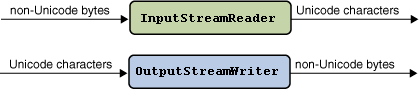
\includegraphics[width=0.75\textwidth]{./inf/SEKII/27_Java_Dateizugriffe/Stream-Kapselung.png}
% http://docs.oracle.com/javase/tutorial/i18n/text/stream.html
% http://docs.oracle.com/javase/tutorial/information/license.html
\end{center}

Sollen hingegen Binärdaten gelesen und geschrieben werden, dann arbeitet man
direkt mit dem \myClass{FileInputStream}- beziehungsweise
\myClass{FileOutputStream}-Objekt (wird bei uns im Unterricht nicht vorkommen).

\subsection{Einlesen von Daten}

Zum Lesen von Daten aus dem Stream besitzt die Klasse
\myClass{InputStreamReader} unter anderem die folgende Methode:

\begin{lstlisting}
public int read() throws IOException
\end{lstlisting}

\lstinline|read()| liest das nächste Zeichen vom Datenstrom ein. Wenn ein
Zeichen übertragen wurde, ist das Ergebnis eine Zahl, die mit einem Type-Cast
in einen Buchstaben (\lstinline|char|) umgewandelt werden kann. Falls keine
Daten verfügbar sind, blockiert die Methode bis das nächste Zeichen angekommen
ist. Wenn die Datenverbindung geschlossen wurde, wird der Wert \lstinline|-1|
zurückgegeben.

\subsection{Ausgabe von Daten}

Zur Ausgabe von Daten besitzt die Klasse \myClass{OutputStreamWriter} unter
anderem die folgenden Methoden:

\begin{lstlisting}
public void write(int zeichen) throws IOException
public void write(String text) throws IOException
\end{lstlisting}

Die obere Variante der \lstinline|write()|-Methode schreibt ein einzelnes
Zeichen in den Datenstrom, die untere Variante schreibt einen String. Die mit
\lstinline|write()| geschriebenen Daten werden zunächst (intern)
zwischengepuffert und erst dann tatsächlich verschickt, wenn der Puffer gefüllt
ist. Mit der Methode \lstinline|flush()| kann man das tatsächliche Versenden
sofort erzwingen:

\begin{lstlisting}
public void flush() throws IOException
\end{lstlisting}

\subsection{Datei schließen}

Am Ende sollte die Datei mit der Methode \lstinline|close()| (anzuwenden auf das
\myClass{FileInputStream}- bzw. auf das
\myClass{FileOutputStream}-Objekt)geschlossen werden:

\begin{lstlisting}
public void close() throws IOException
\end{lstlisting}

Das kann man sich allerdings sparen, wenn man das \myClass{FileInputStream}- bzw
das \myClass{FileOutputStream}-Objekt mit try-with-resource erzeugt (siehe
Beispiel-Code weiter unten).

\section{Dateinamen und -pfade}

Um eine Datei mit \myClass{FileInputStream} bzw.\ \myClass{FileOutputStream} zu
öffnen, muss man ihren Namen angeben. Solange ihr keine Dateien neu erzeugen
müsst (sprich: solange die zu öffnende Datei bereits existiert), empfehle ich
euch folgende Variante:

\begin{lstlisting}
URL url = getClass().getResource("datei.txt");
InputStream is = new FileInputStream(url.getFile());
InputStreamReader in = new InputStreamReader(is, "UTF-8");
\end{lstlisting}

bzw.

\begin{lstlisting}
URL url = getClass().getResource("datei.txt");
OutputStream os = new FileOutputStream(url.getFile());
OutputStreamWriter out = new OutputStreamWriter(os, "UTF-8");
\end{lstlisting}

Das Java-Programm wird dann versuchen die entsprechende Datei im dem
Verzeichnis zu öffnen, in dem auch das Java-Programm gestartet wurde. In
Eclipse also innerhalb des Packages, in dem das Programm liegt. Wenn es die
angegebene Datei nicht gibt, dann wird beim Zugriff über
\lstinline|url.getFile()| eine \myClass{NullPointerException} erzeugt.

Alternativ kann man auch zusätzlich zum Dateinamen den Pfad zur Datei mit
angeben. Entweder als absoluter Pfad wie etwa
\myFile{C:/Users/hartmut/Documents/Datei.txt}\footnote{Der unter Windows
übliche Backslash '\ensuremath{\backslash}' als Pfad-Trenner muss durch einen
Slash '/' ersetzt werden.} oder als relativer Pfad (relativ zum aktuellen
Arbeitsverzeichnis), etwa \myFile{src/dateizugriffe/datei.txt}

Beides hat jedoch Nachteile: Absolute Pfade sind plattformabhängig. Was unter
Windows ein gültiger Pfad ist macht unter MacOS und Linux/Unix keinen Sinn. Und
umgekehrt. Und relative Pfade führen zu unterschiedlichen Ergebnissen, je
nachdem, was das aktuelle Arbeitsverzeichnis ist.

Oder man lässt den Benutzer die Datei mit einem Dateiauswahldialog interaktiv
bestimmen (Siehe die Zusatzaufgabe zu Aufgabe 1 in diesem Kapitel).


\section{Dateien aus JAR Archiven zum Lesen öffnen}

Wenn man Dateien in ein JAR mit einpackt und diese lesen will (braucht ihr im
Unterricht nicht), empfiehlt sich folgende Variante:

\begin{lstlisting}
InputStream is = getClass().getResourceAsStream("notizen.txt");
InputStreamReader fileIn = new InputStreamReader(is, "UTF-8");
\end{lstlisting}

Die im Beispiel benutzte Datei \myFile{notizen.txt} würde gefunden, wenn sie im
gleichen Verzeichnis liegt, wie die aufrufende Klasse. Liegt sie in einem
Unterverzeichnis (relativ zum Verzeichnis, in dem die Klasse liegt) dann würde
man sie entsprechend mit \myFile{unterverzeichnis/notizen.txt} erreichen.

In JAR-Archive kann man jedoch nicht schreiben. Für schreibende Dateizugriffe
(im normalen Dateisystem, nicht in JAR-Archiven) benutzt man deswegen die oben
genannten Methoden.


\section{Beispiel: Schreiben in eine Datei}

\begin{lstlisting}
import java.io.FileOutputStream;
import java.io.IOException;
import java.io.OutputStream;
import java.io.OutputStreamWriter;
import java.net.URL;

public class Schreiben {
	
    public Schreiben() {
        URL url = getClass().getResource("hallo.txt");

        if (url == null) {
            System.out.println("Fehler beim Schreiben: Datei existiert nicht.");
            return;
        }
        try (OutputStream os = new FileOutputStream(url.getFile());
                OutputStreamWriter out = new OutputStreamWriter(os, "UTF-8")) {
            out.write("Heißer Kaffee!" + System.lineSeparator());
            out.flush();
        } catch (IOException e) {
            System.out.println("Fehler beim Schreiben:" + e.getMessage());
        }
    }

    public static void main(String[] args) {
        new Schreiben();
    }
}
\end{lstlisting}


\section{Beispiel: Lesen aus einer Datei}

\begin{lstlisting}
import java.io.FileInputStream;
import java.io.IOException;
import java.io.InputStream;
import java.io.InputStreamReader;
import java.net.URL;

public class Lesen {
	
    public Lesen() {
        URL url = getClass().getResource("hallo.txt");
        int zeichen;
	
        if (url == null) {
            System.out.println("Fehler beim Lesen: Datei existiert nicht.");
            return;
        }
        try (InputStream is = new FileInputStream(url.getFile());
                InputStreamReader in = new InputStreamReader(is, "UTF-8")) {
            while ((zeichen = in.read()) != -1) {
                System.out.print((char) zeichen);
            }
        } catch (IOException e) {
            System.out.println("Fehler beim Lesen:" + e.getMessage());
        }
    }

    public static void main(String[] args) {
        new Lesen();
    }
}
\end{lstlisting}